\section{Prototype}
\label{sec:prototype}
To evaluate the capabilities and modular structure of \textit{Clixon}, a prototype was developed based on the YANG model specified in the RFC draft \textit{ietf-tcpm-yang-tcp}~\cite{draft-ietf-tcpm-yang-tcp}.

In the following subsections, first, the proposed YANG model \textit{ietf-tcp} used in the prototype is introduced. Subsequently, the difficulties encountered during the development of the plugin are outlined. In the last subsection \ref{Portability to QNX} the portability of the prototype and the underlying \textit{Clixon} framework is analyzed based on the Blackberry real-time operating systems (RTOS) QNX and an armv7 system architecture as evaluation platform.

%%%%%%%%%%%%%%%%%%
% IETF TCP YANG Model
%%%%%%%%%%%%%%%%%%
\subsection{IETF TCP YANG Model}
\label{IETF TCP YANG Model}

\begin{figure}[htbp]
    \centering
    \begin{lstlisting}[gobble=8,language={}]
        module: ietf-tcp
         +-rw tcp!
           +-rw connections
           | +-rw connection*
           |   +-rw local-address     
           |   +-rw remote-address    
           |   +-rw local-port        
           |   +-rw remote-port       
           |   +-rw common
           |     +-rw keepalives! 
           |     |  +-rw idle-time         
           |     |  +-rw max-probes        
           |     |  +-rw probe-interval    
           |     +-rw (authentication)?
           |       +-:(ao)
           |       |  +-rw enable-ao?            
           |       |  +-rw send-id?              
           |       |  +-rw recv-id?              
           |       |  +-rw include-tcp-options?  
           |       |  +-rw accept-key-mismatch?  
           |       +-:(md5)
           |         +-rw enable-md5?            
           +-ro statistics {statistics}?
             +-ro active-opens?             
             +-ro passive-opens?            
             +-ro attempt-fails?            
             +-ro establish-resets?         
             +-ro currently-established?    
             +-ro in-segments?              
             +-ro out-segments?             
             +-ro retransmitted-segments?   
             +-ro in-errors?                
             +-ro out-resets?               
             +-x reset
               +-w input
               | +-w reset-at?  
               +-ro output
                 +-ro reset-finished-at?  
        \end{lstlisting}
    \caption{TCP YANG.}
    \label{fig:ietf-yang}
\end{figure}

The TCP Maintenance and Minor Extensions (TCPM) working group of the IETF is currently working on a standardized YANG Model for the TCP stack named \textit{ietf-tcp}~\cite{draft-ietf-tcpm-yang-tcp}. It specifies a minimal YANG model for the TCP stack which is presented in Figure~\ref{fig:ietf-yang}. It consists of a container for all TCP connections and a container for basic TCP statistics. In addition, it defines groupings of authentication parameters that can be reused by other models.

To our knowledge, the presented prototype is the first implementation of the proposed \textit{ietf-tcp} model. However, it must be mentioned that the YANG model could not be implemented to its full extent, since at the time of implementation the functionality required for the authentication container was not supported by the Linux kernel.
Furthermore, the list of TCP connections was only implemented as a read-only list because write access was not applicable in the prototype environment.
Likewise, the reset action for the TCP statistics could not be implemented properly due to the lack of support provided by the operating systems used (Ubuntu, QNX).

Nevertheless, the evaluation phase provided valuable insights that contributed to the further development of the YANG model~\footnote{Further information about changes to the YANG model and the contribution of this work can be found in the slide decks for IETF 110~\cite{ietf-110} and IETF 111~\cite{ietf-111}.}.


%%%%%%%%%%%%%%%%%%
% Plugin Development
%%%%%%%%%%%%%%%%%%
\subsection{Plugin Development}
\label{Plugin Development}

\begin{figure}[h!]
    \centering
    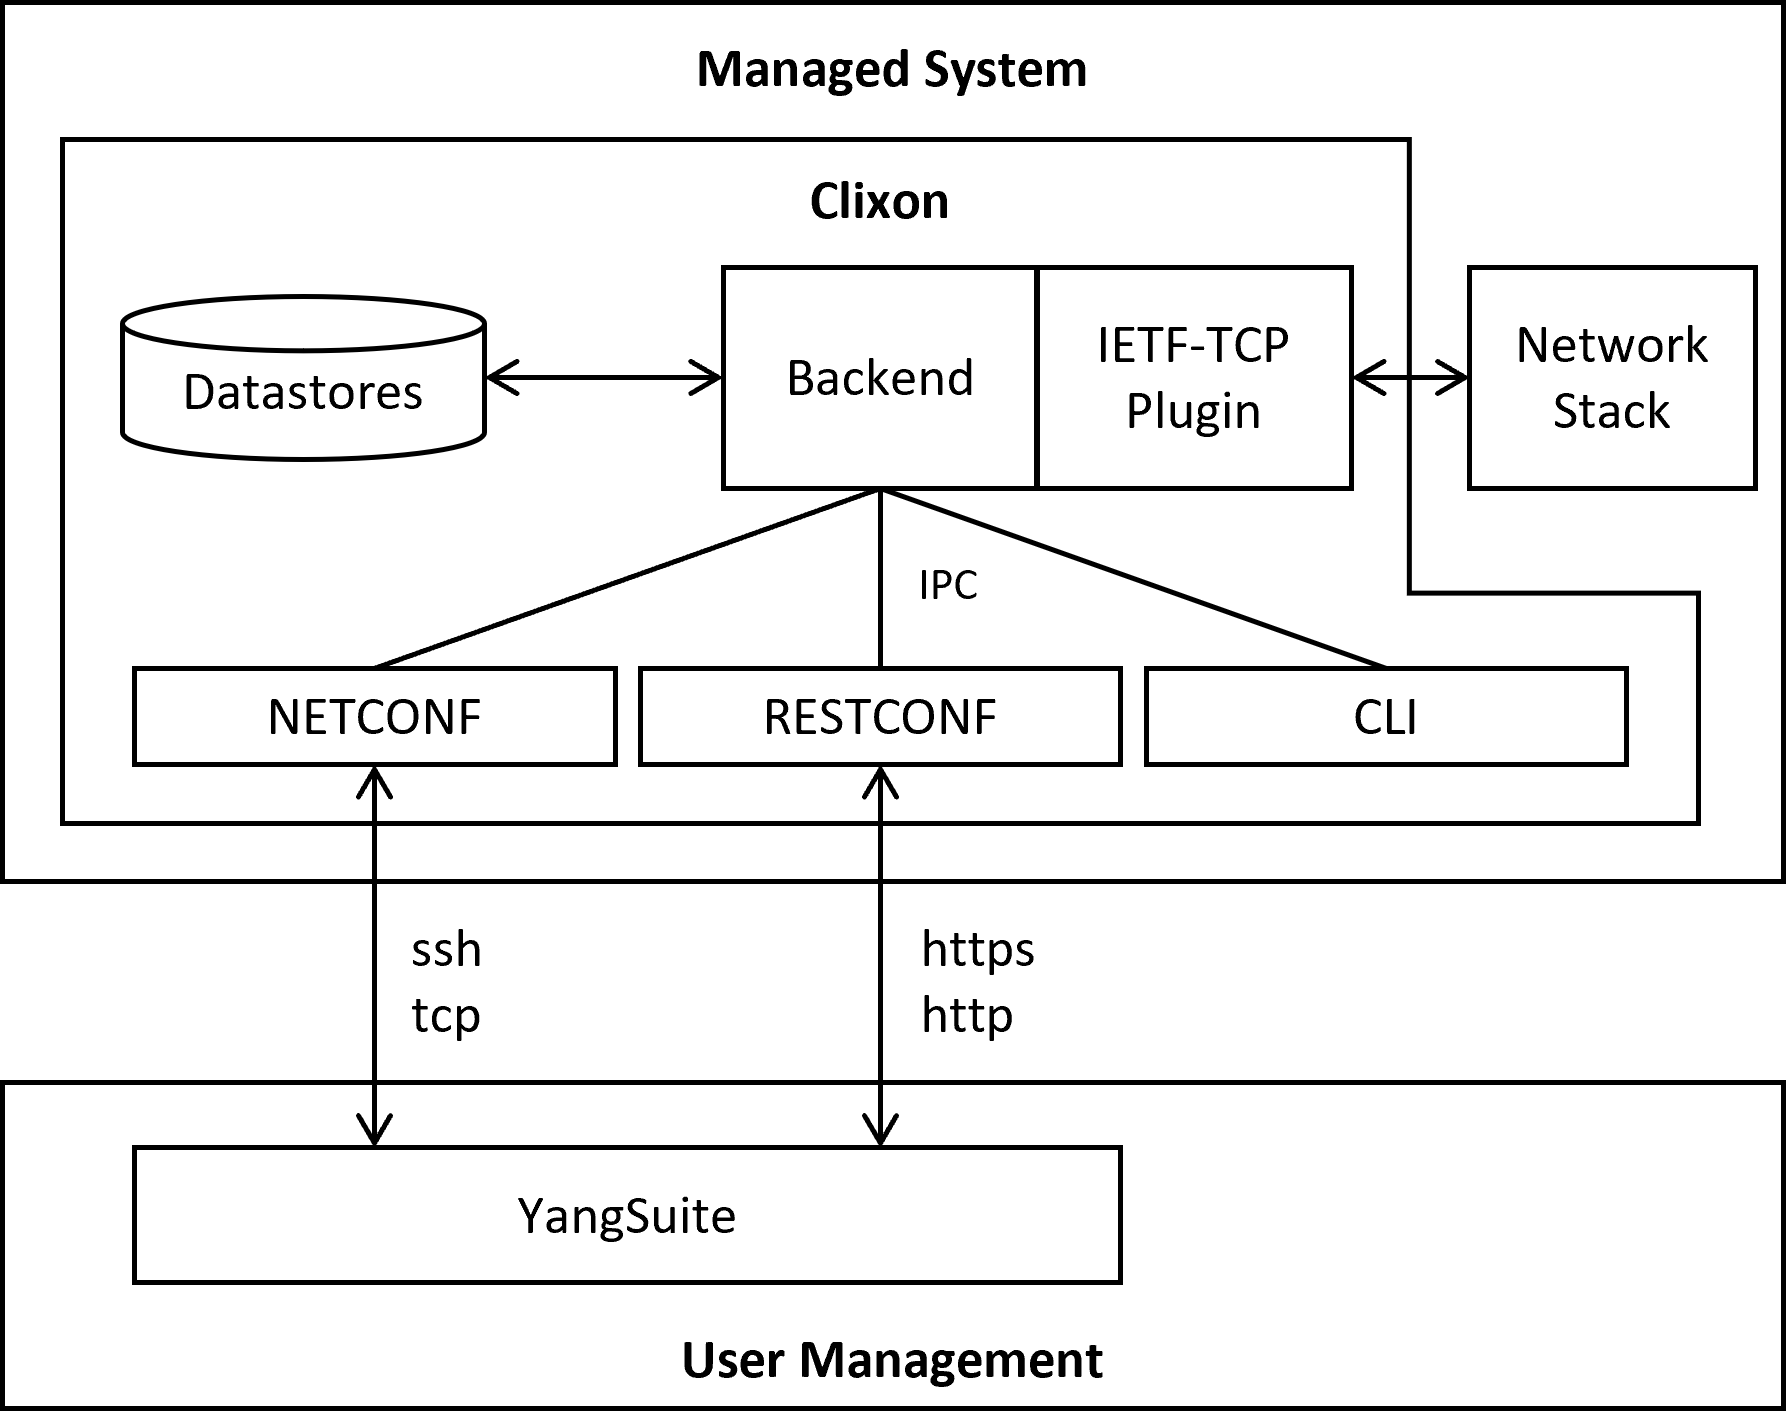
\includegraphics[width=\linewidth]{assets/Prototype/Plugin_Architecture_v.png}
    \caption{Plugin Architecture}
    \label{fig:plugin_architecture}
\end{figure}

Unlike the \textit{Clixon} framework, which is written entirely in \inlinelst{C} and based on the \textit{Autotools toolchain} as the build system, the plugin was developed using \inlinelst{C++} and \textit{CMake} for better development experience.

To obtain the TCP connections and statistics specified in the YANG model from the base system, in this case Ubuntu, the pseudo files \inlinelst{/proc/net/snmp} and \inlinelst{/proc/net/tcp} were read and parsed.

For testing the implementation of the plugin, \textit{YangSuite} was used, which was fairly new at the time of implementation. It provides interfaces like NETCONF and RESTCONF gNMI and and can be operated in a docker container. Fig.~\ref{fig:plugin_architecture} shows how \textit{YangSuite} integrates into the user management layer and into the overall setup.

The Source code for the implemented plugin can be found on GitHub at https://github.com/mager-m/ietf-tcp-research-project.

%%%%%%%%%%%%%%%%%%
% Portability to QNX
%%%%%%%%%%%%%%%%%%
\subsection{Portability to QNX}
\label{Portability to QNX}

% Why QNX?
QNX is a commercially distributed real time operating system (RTOS) that is used through various industries and serves as the basis in many embedded devices, including network related equipment. Therefore QNX has been chosen as the evaluation platform for the portability analysis. A physical development board, based on the ARMv7 architecture, has been used in the process.

% Technical Prerequisites -> Port Effort 
Since \textit{Clixon}'s goal is to provide a YANG-based configuration manager with support for many platforms, it already runs on a variety of operating systems. To achieve this, \textit{Clixon} relies on different feature flags and the use of \textit{Autotools toolchain} to detect the platform capabilities at configuration time. This not only made it easier to get the framework up and running, but also to adapt any necessary changes as described in the following. 

%& Findings + Challenges
% CLixon
During the deployment of the framework to the new platform a memory corruption appeared while reading the YANG models from the disk. Presumably due to a different memory management it has not been noticed with Ubuntu so far. An appropriate fix was implemented and merged in agreement with the maintainer into the project as pull request.

Another challenge was the lack of support for the multiple privilege functions such as \inlinelst{setresuid} and \inlinelst{getresuid} that are used by \textit{Clixon} to drop privileges after initialization. To overcome this issue, an additional check in \textit{Autotools} along with the feature flag \inlinelst{HAVE\_SETRESUID} was introduced. Thus, if \inlinelst{getresuid} / \inlinelst{setresuid} is not available on the platform, it will be detected during the configuration phase and the relevant code will not be included in the compilation. This change was also merged into the project with a pull request. 

Due to the highly generic code structure, the deployment of the \textit{Clixon} framework to the evaluation platform proceeded without further challenges.

% Plugin
Since QNX does not have the same pseudo files for reading TCP connections and statistics as Ubuntu, modifications to the plugin were necessary. To overcome the non-existent files, the information was obtained by using the \inlinelst{netstat} command and parsing the corresponding output. Otherwise, no major changes were necessary.
    
% Fazit
The deployment of the prototype to the evaluation platform has confirmed the initial assumption and the advertisement of \textit{Clixon}. Due to the generic code base and the use of the \textit{Autotools toolchain} along with many feature flags, the framework proved to be very flexible and easily portable to new UNIX-like environments.

The various challenges faced during the deployment have also highlighted the benefits of open-source software. Besides the possibility to make changes directly to the source code, there is a solid community for emerging questions during the development. Since the changes can be contributed and merged, the framework is constantly evolving and so are the capabilities.

% 
%Since model-based management is also becoming increasingly important in other industries beyond traditional network management, the portability of the implemented software solution was evaluated subsequently.
